    \section{Gebruikershandleiding}
    \label{app:handleiding}
    \emph{Grudge of the Oblivious} speelt zich af in een oorlog tussen twee rivaliserende robot-bendes. Het spel is voor meerdere spelers, elke speler speelt een robot uit \'e\'en van deze twee robot-bendes. Elke robot-bende heeft zijn eigen commandocentrum. Het doel van het spel is om het commandocentrum van de andere robot-bende te vernietigen.

    Robots hebben krachtige lasergeweren om andere robots te vernietigen en gebouwen aan te vallen. Deze lasergeweren hebben een bepaald bereik. Als een robot schiet op een object die verder dan dit bereik van de speler af staan wordt er een laserstraal afgevuurd die het object niet bereikt. Gebouwen kunnen door spelers worden neergezet op het terrein. Hiervoor moet echter wel goud worden betaald. Je kan goud verdienen voor de gezamenlijke kas van de robot-bende door mijnen te bouwen over delfplaatsen. Verder kan goud worden verdiend door robots of gebouwen uit de andere robot-bende te vernietigen. Als een speler dood gaat of een gebouw wordt vernietigd, zullen muntjes worden achtergelaten. Dit muntje kan vervolgens door alle spelers worden opgepakt om de gezamenlijke kas te spekken.

	\subsection{Installatie eisen}
	Om het spel te kunnen spelen zijn er een bepaald aantal eisen:
	\begin{itemize}
		\item De computer moet een van de volgende besturingsystemen draaien: Windows XP of hoger, Mac OS X 10.6 of hoger, Linux;
		\item Op de computer moet een grafische kaart hebben met OpenGL ondersteuning.  De minimale eisen voor de grafische kaart is, dat deze vergelijkbaar (of beter) is met de prestaties van een Intel HD graphics 3000;
		\item Een juist ge\"installeerde driver voor de grafische kaart;
		\item Een processor vergelijkbaar met Intel Core 2 Duo op 2 GHz;
		\item In het geval dat het besturingsysteem Mac OS X is, moet de nieuwste versie van X11 of XQuartz ge\"installeerd zijn. Deze is te vinden op \url{http://xquartz.macosforge.org/trac/wiki/Releases}
	\end{itemize}

	\subsection{Terrein}
    Aangezien het spel gedeeltelijk in het genre RTS valt, speelt het terrein een grote rol. Het terrein is, zoals in figuur \ref{fig:terrein} is te zien, volledig symmetrisch. Beide commandocentra staan aan de rand van het terrein. Standaard staan er twee torens bij de commandocentra ter verdediging. De verschillende delfplaatsen zijn licht grijs in het figuur. Er zijn bovendien nog drie extra rijke delfplaatsen. Deze zijn midden links, midden rechts en in het midden geplaatst. Het verschil tussen deze twee type delfplaatsen zullen we zo nog uitleggen.

    \begin{figure}[h]
        \centering
    	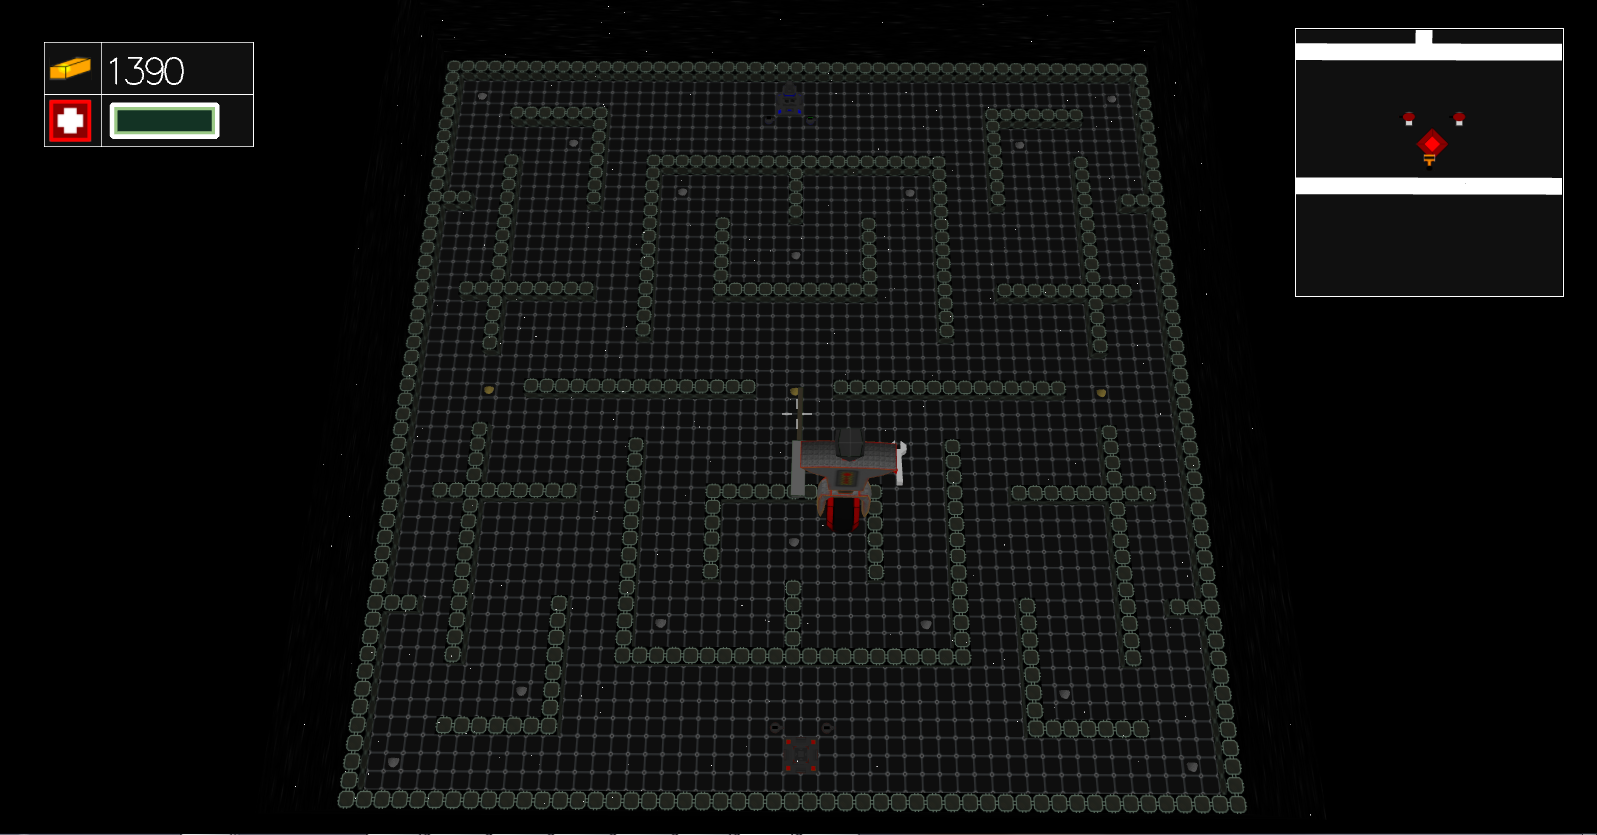
\includegraphics[width=\textwidth]{kaart.png}
	\caption{Een bovenaanzicht van het spel}
    \label{fig:terrein}
    \end{figure}

    \subsection{Spelers}
    De verschillende robot-bendes zijn te onderscheiden door kleuren. Zo is er een team Rood en een team Blauw. Standaard zit je in team Rood. Dit kan als volgt worden aangepast. Druk eerst op \textsc{Enter} en typ \textsc{set team b} in kleine letters. Vanaf dat moment zit je standaard in team Blauw: dit zal in werking treden als je het spel opnieuw opstart. Dit kan weer worden teruggedraaid door \textsc{set team a}.

    Je ziet de wereld vanuit de positie van je robot. De kijkrichting kan in elke willekeurige richting worden aangepast. Je robot zal dan meedraaien met de kijkrichting. Als de robot naar voren beweegt, zal de robot geleidelijk naar de kijkrichting draaien. Bij het schieten zal de laserstraal altijd in de huidige kijkrichting worden afgevuurd. De laserstraal heeft echter maar een beperkt bereik.

    Elke robot heeft een harnas. Bij het begin van het spel heeft de robot nog een volledig harnas. Zodra de speler wordt geraakt, wordt de conditie van het harnas slechter. Hierbij is grote voorzichtigheid vereist: je kan namelijk ook het harnas van andere leden uit jouw bende beschadigen. Een robot gaat dood als zijn harnas kapot is. In dat geval zal hij na een bepaalde hoeveelheid tijd terugkeren bij het commandocentrum met een volledig harnas.

    Je kan op het grondvlak vooruit en achteruit bewegen met een vaste snelheid. Je kan draaien door de kijkrichting aan te passen. Hierbij moet je natuurlijk op de kaart blijven. Ook kan je niet door gebouwen lopen. Het is wel mogelijk dat spelers door elkaar lopen. Je bestuurt het spel vanuit een derde persoon perspectief. Dit betekent dat je het spel bekijkt vanaf een punt vlak achter de speler. Het is bovendien mogelijk om te wisselen naar een eerste persoon perspectief door te \emph{scrollen}.

    \subsection{Gebouwen}
    Er zijn drie soorten gebouwen: torens, mijnen en commandocentra. Het bouwen van een toren kost 200 eenheden aan goud. Torens schieten op spelers en gebouwen van de andere robot-bende in hun bereik. Merk op dat torens een groter bereik hebben dan je eigen robot. Torens kunnen overal worden geplaatst onder de voorwaarde dat er nog geen ander gebouw of delfplaats staat op die plek. Mijnen kunnen over delfplaatsen worden gebouwd met het doel de inkomsten van een team te vergroten.

    Er zijn twee typen deflplaatsen, normale en extra rijke delfplaatsen. Het bouwen van een mijn over een normale delfplaats kost 220 eenheden aan goud. Het bouwen van een mijn over een extra rijke delfplaats kost 320 eenheden aan goud. Een mijn, die over een normale delfplaats is geplaatst, levert periodiek 30 eenheden aan goud op. Een mijn, die over een extra rijke delfplaats is geplaatst, levert periodiek 60 eenheden aan goud op. Deze periode is gelijk voor beide delfplaatsen. Het veroveren van een extra rijke delfplaats kan dus van groot belang zijn om het spel te winnen.

    Het commandocentrum is het belangrijkste gebouw van een robot-bende: het levert bovendien periodiek 10 eenheden aan goud op. Als dit gebouw wordt vernietigd, heeft het bijbehorende team verloren. Gebouwen kunnen door spelers worden beschoten, waardoor deze worden beschadigd. Bij voldoende schade zal het gebouw worden vernietigd. Dan kan op deze plaats, indien gewenst, een ander gebouw worden geplaatst. Gebouwen kunnen ge\"identificeerd worden door de kleur van het gebouw, dat correspondeert met de kleur van het team.

    \subsection{Verzamelbare voorwerpen}
    Er is maar \'e\'en verzamelbaar voorwerp: een muntje. E\'en of meerdere muntjes worden achtergelaten door spelers die dood gaan en torens die worden vernietigd. Als een speler dood gaat, is de totale waarde van de muntjes gelijk aan de gezamenlijke kas van dat team gedeeld door twee keer het aantal spelers in het team. Als een gebouw wordt vernietigd, dan is de totale waarde van de muntjes gelijk aan de helft van de kosten voor dat gebouw.

    Een muntje is 20 eenheden in goud waard. Aangezien we natuurlijk altijd een geheel aantal muntjes achterlaten, zullen we indien nodig naar beneden afronden. Als een speler doodgaat, wordt bovendien nog de waarde van de muntjes afgetrokken van de gezamenlijke kas van die speler. Een muntje kan vervolgens opgepakt worden door alle spelers. De waarde van het muntje zal dan toegevoegd worden aan de kas van het bijbehorende team.

    \subsection{Initialisatie}
	Om het spel op te starten kan je simpelweg het spel openen. Dan zit je in een spel met \'e\'en speler, namelijk jezelf. Om een multiplayer spel op te starten heb je meerdere mogelijkheden, of je laat andere spelers met jezelf verbinden, of je verbind met andere spelers. Om met andere spelers te verbinden druk je de knop \textsc{Enter} in en typ je \textsc{Discover}. Op je scherm staan nu alle spelers die in hetzelfde subnet zitten als jezelf. 
	
	Je kan nu aan het spel meedoen door het nummer van \'e\'en van deze spelers te onthouden. Dit nummer staat voor de speler. Druk nu weer op de knop {Enter} en typ in \textsc{Join} gevolgd door een spatie en het nummer van een speler. Nu kan je meedoen aan hetzelfde spel als die speler.
	
    Bij de start van het spel staan alle spelers bij het commandocentrum. Zoals al eerder gezegd, hebben alle spelers dan nog een volledig harnas. Bovendien zit er dan voor 200 eenheden aan goud in de kas.

    \FloatBarrier

    \subsection{Besturing}
    \label{sec:UI}

    Naast het spel kan je het volgende op je scherm zien:
    \begin{itemize}
    \item De hoeveelheid goud van het team, deze hoeveelheid staat achter een goudstaaf.
    \item De sterkte van het harnas, die wordt weergegeven door middel van een statusbalk.
    \item Het vizier van de speler.
    \item Een plattegrond.
    \end{itemize}

    Je vizier wordt altijd in het midden van het scherm geplaatst. Het mikken met het vizier gebeurt dus door het veranderen van de kijkrichting. De speler wordt altijd iets links van dit vizier getekend. Voor de duidelijkheid hebben wij hier ook een figuur van gemaakt, zie figuur \ref{fig:UI}.
    \begin{figure}
    \includegraphics[width=0.9\textwidth]{../Graphics/UI.eps}
    \caption{De gebruikersomgeving tijdens het spel}
    \label{fig:UI}
    \end{figure}
    De besturing van de robot kan met de \textsc{wasd}-toetsencombinatie of door gebruik te maken van de pijltjes-toetsen. Hiervoor geven we de volgende tabel:
    \begin{table}[H]
        \small
        \centering
        \begin{tabular}{| l | l |}
        \hline
        Knop & Reactie \\ \hline
        \textsc{w} of $\uparrow$ & De robot beweegt, indien mogelijk, vooruit naar de huidige kijkrichting toe \\ \hline
        \textsc{a} of $\leftarrow$ & De robot draait naar links \\ \hline
        \textsc{s} of $\downarrow$ & De robot beweegt, indien mogelijk, achteruit van de huidige kijkrichting af \\ \hline
        \textsc{d} of $\rightarrow$ & De robot draait naar rechts \\ \hline
        \end{tabular}
        \caption{Knoppen met bijbehorende reactie}
        \label{tab:planning}
    \end{table}

    Het is belangrijk om te beseffen dat \textsc{a} of \textsc{d} alleen de richting van de robot aanpassen. Je robot rijdt op een wiel, dus dit kan natuurlijk alleen als de robot al naar voren of naar achteren aan het bewegen is. De kijkrichting kan worden aangepast door gebruik te maken van de muis. Door de muis naar boven of naar beneden te bewegen, kijkt de speler verder omhoog of omlaag respectievelijk. Op analoge wijze kan de speler naar links of naar rechts draaien door respectievelijk de muis naar links of naar rechts te bewegen.

    De speler kan schieten door op de linkermuisknop te drukken. Merk op dat het vizier altijd in het midden van het scherm blijft. Hierdoor is een directe correspondentie tussen muis, vizier en kijkrichting. We tekenen daarom ook geen muis in het scherm. Deze kan worden losgekoppeld door op de rechtermuisknop te drukken. Chatten is in het spel mogelijk door \textsc{t} te drukken. De tekst kan vervolgens worden verstuurd door \textsc{Enter} te drukken.

    \subsection{Het neerzetten van gebouwen}
    Om een gebouw neer te zetten moet je eerst op de knop \textsc{b} drukken. Dan ga je in de zogenaamde \emph{bouw-modus}. Er wordt dan op de ondergrond een rooster getekend. Door middel van het vizier kan je een plek op het rooster aanwijzen. Je kan door te klikken dan de opdracht geven om het gebouw neer te laten zetten. Op dat moment wordt de bijbehorende hoeveelheid goud uit de gezamenlijke kas gehaald. Vervolgens zal het gebouw uit de grond verrijzen. Na het neerzetten van het gebouw blijf je in de bouw-modus. Door nogmaals op de knop \textsc{b} te drukken ga je weer uit de bouw-modus. Dit kan gezien worden in figuur \ref{fig:gebouw}.

    \begin{figure}
    \centering
    \includegraphics[width=\textwidth]{../Graphics/UI2.pdf}
    \caption{Een voorbeeld van het neerzetten van een gebouw in de gebruikersomgeving}
    \label{fig:gebouw}
    \end{figure} 